\section{Introduction}

The end of classical device scaling means that the power per unit area on chip
is rising with each technology generation.  This implies that architectures for
future technology nodes will not be able to power-on all components of the chip
simultaneously, with some estimates being 50\% ``dark silicon'' by
8nm~\cite{isca11:dark-silicon}, which is less than 10 years away.  This trend,
the utilization wall, will curtail expected performance improvements.
Interestingly, much of the core's energy is not expended in the functional
units, but rather in the power-hungry structures needed for
attaining reasonable performance on general purpose workloads.  To exploit this,
architects have in part turned to hardware specialization and
accelerators, which sacrifice generality for efficiency in executing either
specific computations or computations for certain application domains.

The slowing of Moore’s law and Dennard scaling has also led a trend towards 
domain specific accelerators (DSAs) for performance and energy consumption~\cite{1815968}. 
DSAs are high performance computation engines for a specific domain. 
In essence, DSAs trade obsoletion for performance and energy efficiency. 
DSAs employ common specialization principles for concurrency, computation, 
communication, data reuse, and coordination, 
but sacrifice programmability completely. 
~\cite{nowatzki2016pushing} shows that a specialized architecture can be developed for 
general purpose programmability and be competitive 
against DSAs by trading only up to 3.8x in area and 4.1x in power. 

\paragraph{}This project tries to explore one such general purpose programmable
accelerator architecture which tries to target different possible program regions.
The idea behind a scalable, programmable and parallel execution hardware is that programmer
can explicitly shard the data into multiple partitions and the computation can happen in parallel 
across these partitions which enable orders of magnitude of performance. Figure~\ref{fig:abs}
shows the ideal programmer needed abstraction to map the computation kernels to the partitioned data
without any conflicts or explicit synchronization primitives. So, our goal in the project is to explore this
parallel programming design space and see what are some lessons we can learn from this exercise w.r.t programming model
and the parallel hardware itself.


\begin{figure}[h]
  \begin{center}
    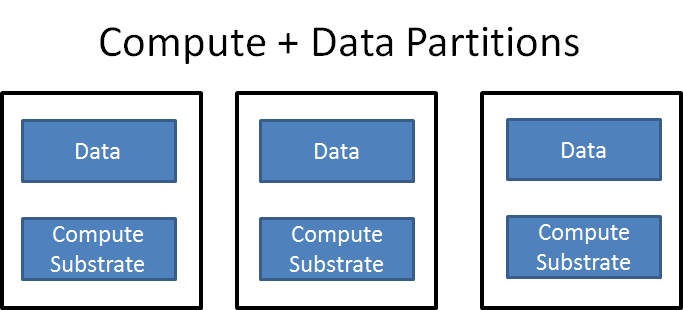
\includegraphics[width=0.65\linewidth, height=2in]{cs758-figs/abstraction.png}
  \end{center}
\vspace{-0.2in}
  \caption{Data and Task Locality for Parallelization}
  \label{fig:abs}
\vspace{-0.4in}
\end{figure}


\paragraph{Document Overview}

Section~\ref{sec:prior} describes the prior work on which the project is based on, 
and how it is resurfaced and remodeled for the project purposes.
Section~\ref{sec:motiv} motivates the need of architectures like proximate and describes the
insights and mechanisms of parallelization on proximate. 
Section~\ref{sec:arch} explains the high level architecture and programming overview of proximate. 
Section~\ref{sec:prog} details over the parallel programming model of proximate and its API calls. 
Section~\ref{sec:meth} explains the methodology used for our project and Section~\ref{sec:eval} explains the results obtained and the corresponding analysis.
We finally end with conclusion in Section~\ref{sec:conc} and future work needed. 


